\subsection{Winkelmodulation (FM/PM) S. 60}
Besser Störfestigkeit aber grösserer Bandbreitenbedarf als AM.

\begin{minipage}{.45\linewidth}
	Äquivalente Basisbanddarstellung der Grosshubwinkelmodulation
	\newline
	
	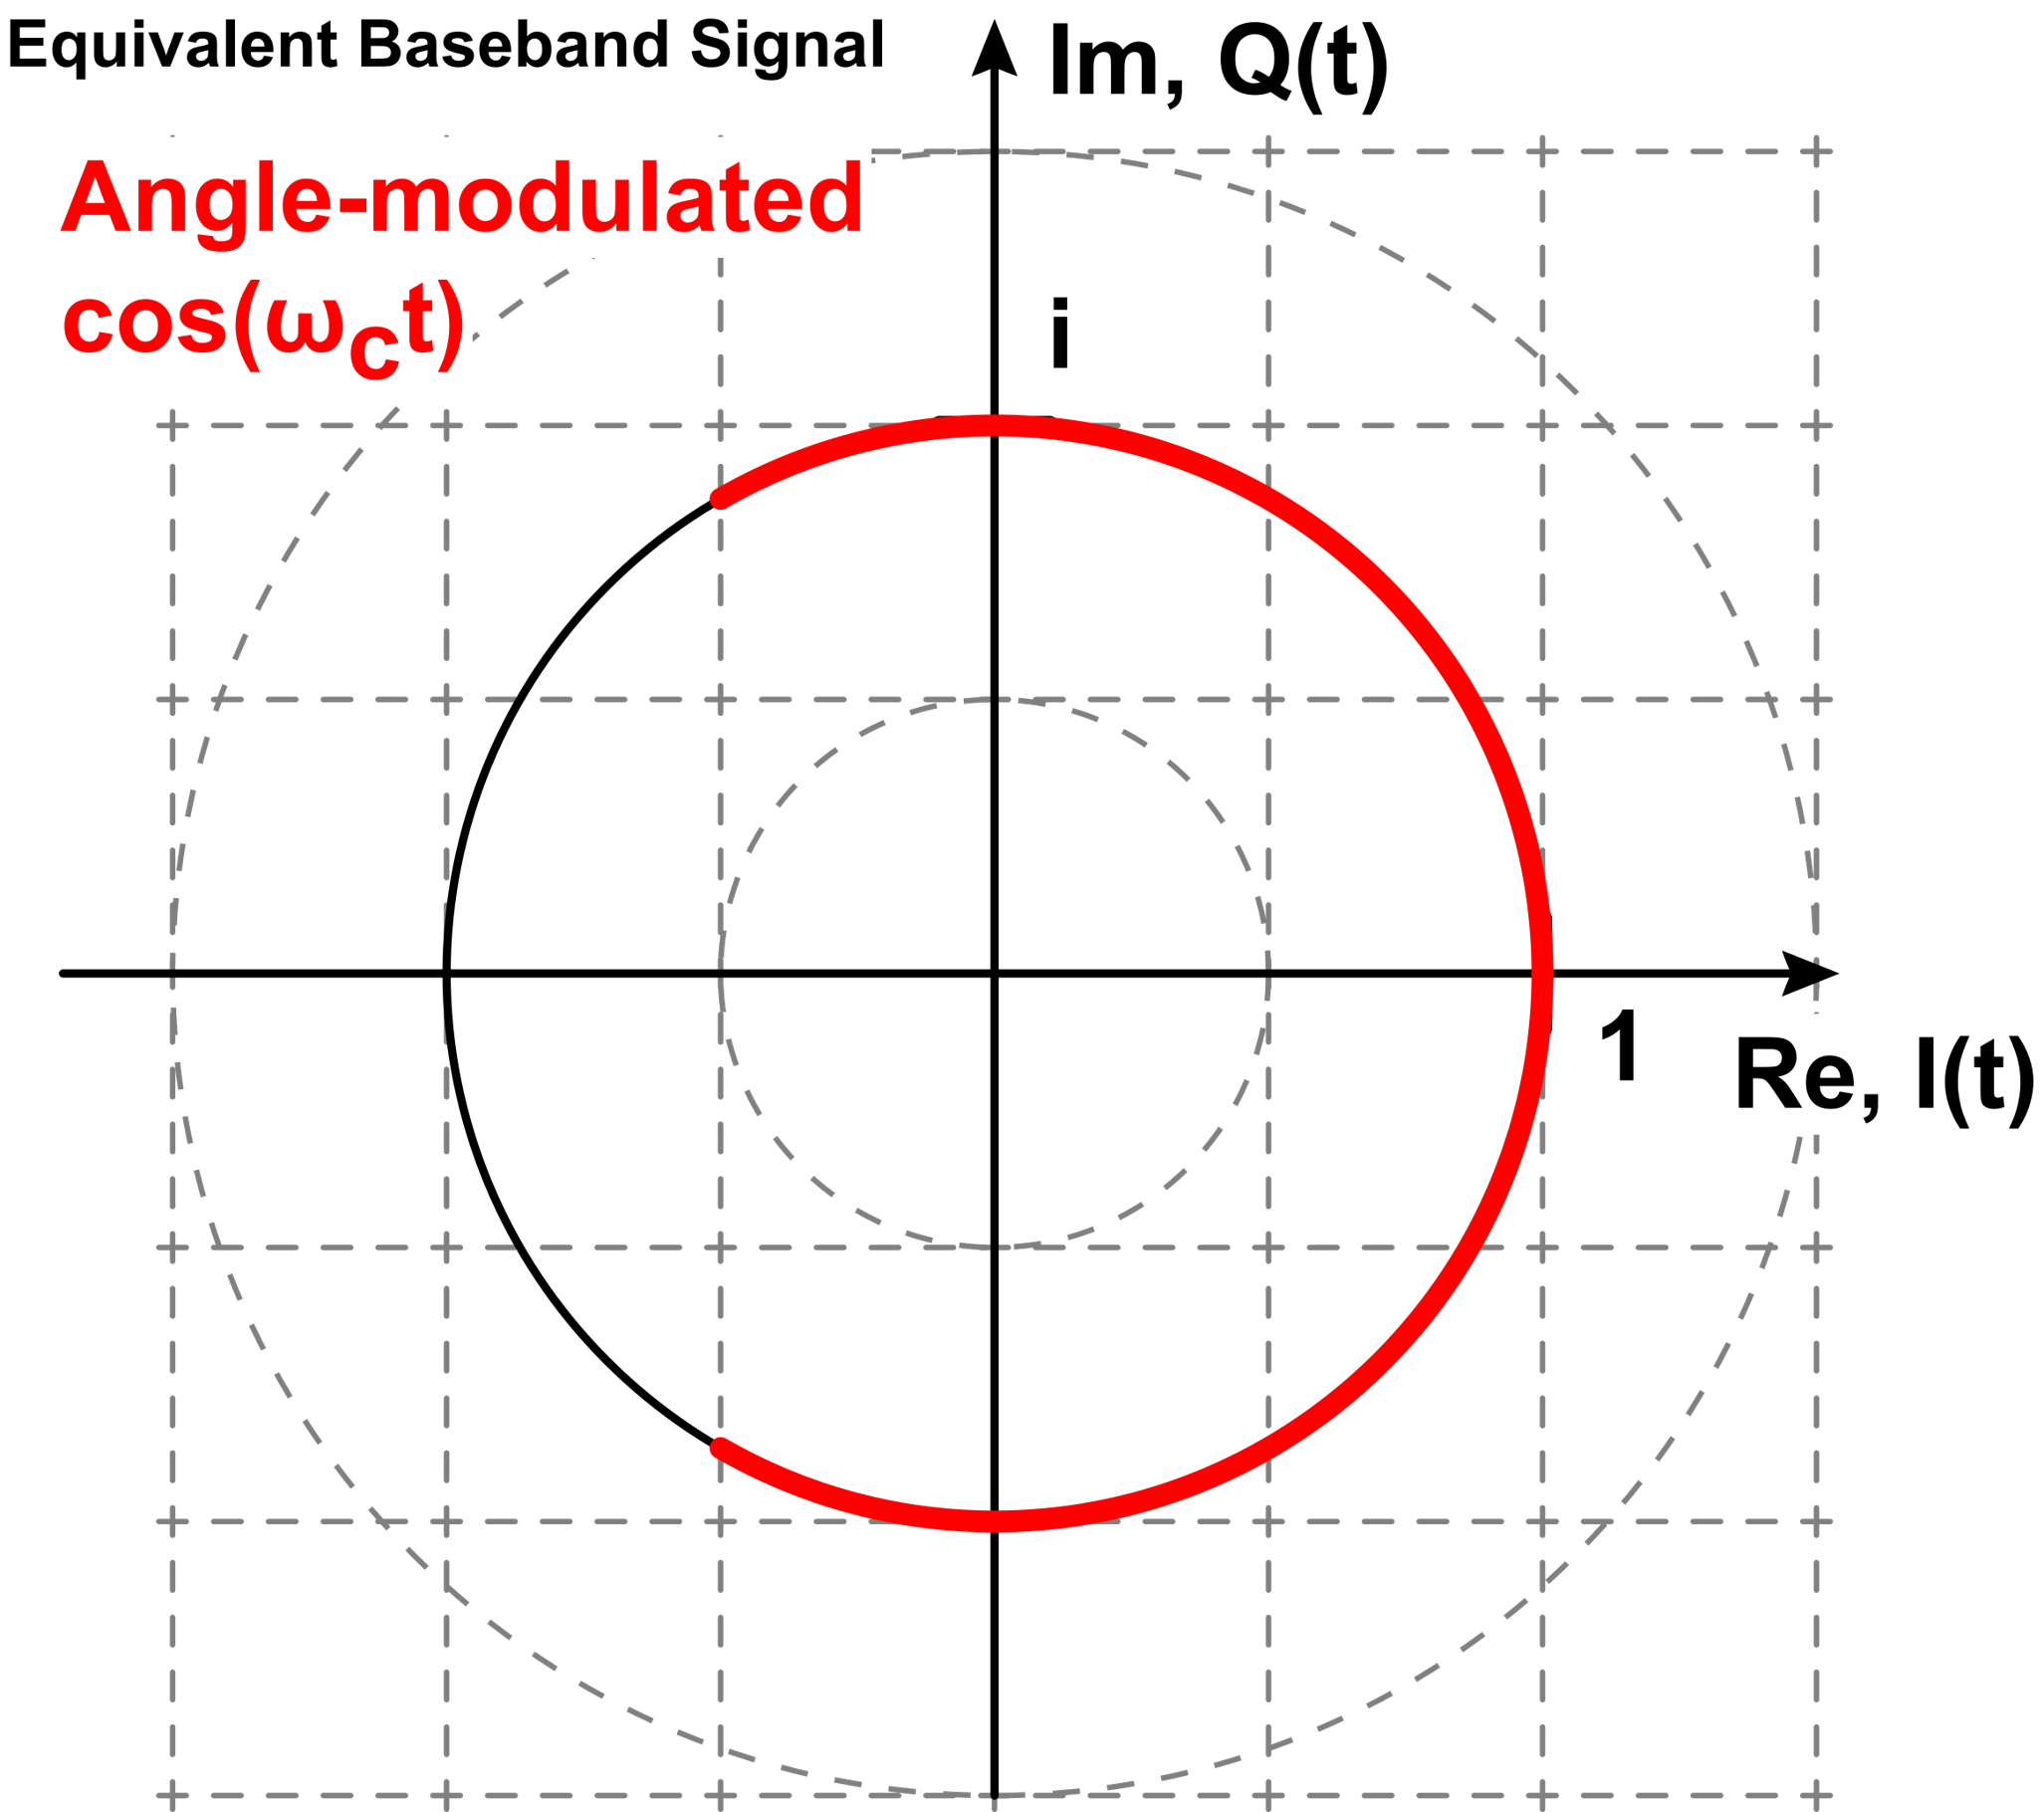
\includegraphics[width=.6\linewidth]{content/06_amplitudenmodulation/PM_zeiger.png}
\end{minipage} \hspace{.1\linewidth}
\begin{minipage}{.45\linewidth}
	
	Zeigerdiagramm des winkelmodulierten Trägersignals
	
	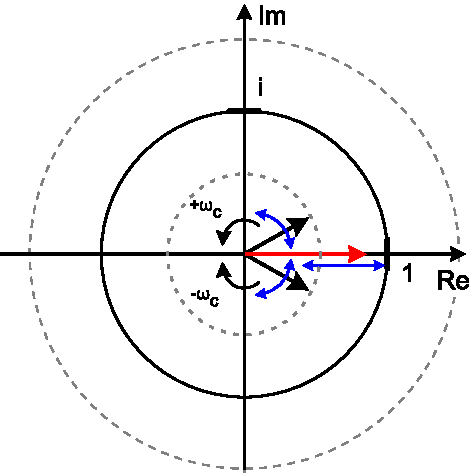
\includegraphics[width=.6\linewidth]{content/06_amplitudenmodulation/abbildung5_26.pdf}
\end{minipage}

\begin{table}[H]
	\begin{tabularx}{\linewidth}{m{.38\linewidth} m{.26\linewidth} m{.3\linewidth}}
		\begin{minipage}{.95\linewidth}
			\textbf{Phasenmodulation PM}\\
			$m(t)$ $\sim$ Phasenabweichung zum Referenzträgersignal\\
			\boxedeq{ \begin{split}
				x_{PM}(t)=A_c\cdot cos(\omega_c t + k_pm(t))\\
				k_p = \text{Phasenhubkonkstante [rad]} \\
				k_p = 2\pi \cdot  \frac{t_{delay,max}}{T_c}
			\end{split}
			}
		\end{minipage}

	&
	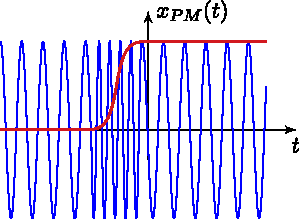
\includegraphics[width=\linewidth]{content/06_amplitudenmodulation/xpm.pdf}
	&
	\begin{minipage}{\linewidth}
		Momentane Phasenabweichung\\
		\efbox[linecolor=red]{$\varphi(t) = k_P \cdot m(t)$}\\
		Momentane Frequenzabweichung \\
		\efbox[linecolor=red]{$ \frac{d\varphi(t)}{dt} = k_P \cdot \frac{dm(t)}{dt}$}\\
		Momentane Frequenz\\
		\efbox[linecolor=red]{$\omega_i(t)=\omega_c+\frac{d\varphi(t)}{dt}$}\\
		Maximale Frequenzabweichung (z.B. bei Jitter)\\
		\efbox[linecolor=red]{$ \Delta \omega = \max( \frac{d\varphi(t)}{dt}) $}
	\end{minipage}
	\\
	\begin{minipage}{.95\linewidth}
		\textbf{Frequenzmodulation FM}\\
		$m(t)$ $\sim$ Frequenzabweichung zum Referenzträgersignal\\
		\boxedeq{\begin{split} x_{PM}(t)=A_c\cdot cos(\omega_c t + k_F\int m(\tau)d\tau)\\
				k_F = \text{Frequenzhubkonkstante [rad/s]} \\
				\frac{A_{k_F} \cdot mpk}{\omega_m} = \varphi_peak(t) \cdot \frac{2\pi}{360} 			
		\end{split}}
	\end{minipage}
	&
	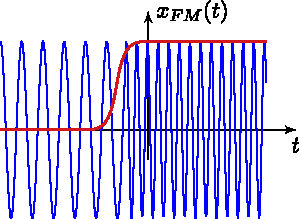
\includegraphics{content/06_amplitudenmodulation/xfm.pdf}
	&
	\begin{minipage}{\linewidth}
		Momentane Phasenabweichung\\
		\efbox[linecolor=red]{$\varphi(t) = k_F \int m(\tau)d\tau$}\\
		Momentane Frequenzabweichung \\
		\efbox[linecolor=red]{$ \frac{d\varphi(t)}{dt} = k_F \cdot m(t)$}\\
		Momentane Frequenz\\
		\efbox[linecolor=red]{$\omega_i(t)=\omega_c+k_F \cdot m(t)$}\
	\end{minipage}
	\end{tabularx}
\end{table}

\subsubsection{Äquivalenz PM und FM}
PM und FM können äquivalent realisiert werden (mit zusätzlichem Integrator oder Differenziator)\\
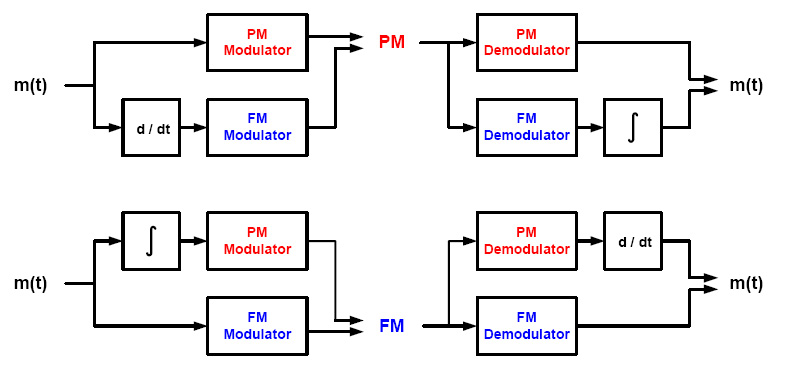
\includegraphics[width=\linewidth]{content/06_amplitudenmodulation/PMundFM.png}

\subsubsection{Spektrum der Winkelmodulation S. 62}
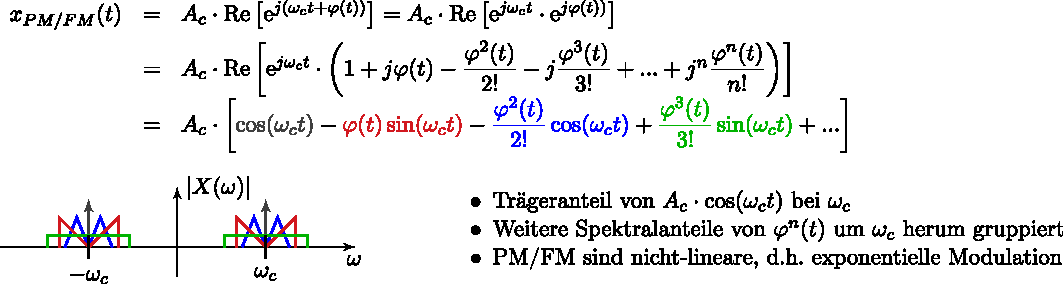
\includegraphics[width=\linewidth]{content/06_amplitudenmodulation/spektrumWinkelmodulation.pdf}

\subsubsection{Kleinhub Winkelmodulation S. 62}
\begin{table}[H]
	\begin{tabularx}{\linewidth}{m{.65\linewidth} m{.35\linewidth}}
		\begin{minipage}{\linewidth}
				Kleinhubmodulation funktioniert in der Praxis bei ca: \efbox[linecolor=red]{$|\varphi(t)| < 0.2 \text{ rad}$} bzw. 10 bis 12 Grad. \\
				Dann gilt: \efbox[linecolor=red]{$x_{NB\phi M}(t) \approx A_c \cdot cos(\omega_c t) - A_c \cdot (\varphi(t)\cdot sin(\omega_ct))$} \\
				\textbf{Demodulation:} mit kohärentem Produktdetektor\\ $\rightarrow x_{NB-PM/FM}(t)\cdot (-sin(\omega_c t))$ \\
				Bild rechts: äquivalente Basisbanddarstellung des Signals\\ $x_{NB-PM}(t) = 0.05 \cdot \sin(2\pi \cdot 200 t) + 1\cdot \sin(2\pi \cdot 1000 t)$\\
				Wobei nur spannend ist, dass die Signalamplitude im Vergleich zur Trägeramplitude sehr klein ist und der Träger eine Sinusschwingung ist (siehe Formeln zu beginn des Kapitels)
		\end{minipage}
		&
		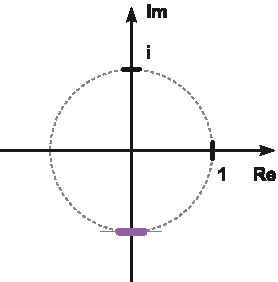
\includegraphics[width=.8\linewidth]{content/06_amplitudenmodulation/eqBase_NBAM.pdf}
	\end{tabularx}
\end{table}

\paragraph{Spektrum S. 62}
\includegraphics[width=.8\linewidth]{content/06_amplitudenmodulation/SpektrumNB_PM.pdf}\\
\textbf{Vergleich AM und NP-PM:} Qualitativ gilt für die Amplitudenspektren $|X_{AM}(\omega)| = |X_{NBPM(\omega)}$

\subsubsection{Grosshub Winkelmodulation S. 63}
WideBand Angle Modulation, siehe auch  Skript Seite 67 \hspace{.3cm} \efbox[linecolor=red]{$|\varphi (t)| > 1$}
	\begin{list}{$\bullet$}{\setlength{\itemsep}{0cm} \setlength{\parsep}{0cm} 	\setlength{\topsep}{0cm}} 
	\item nicht lineare Terme von $\varphi (t)$ nicht mehr vernachlässigbar
	\item analytische Bestimmung des Spektrums nur noch für Eintonsignale durchführbar
	\item Überlagerungssatz nicht mehr gültig
	\item $x_{FM/PM}$ ist zu $m(t)$ stark nicht linear
	\item im Frequenzspektrum treten $\sim m(t)$ Anteile auf
\end{list}
\begin{table}[H]
	\begin{tabularx}{\linewidth}{m{.7\linewidth} m{.3\linewidth}}
		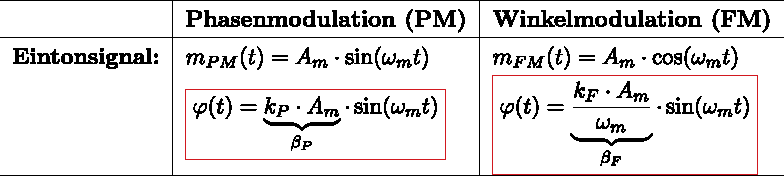
\includegraphics{content/06_amplitudenmodulation/WB_PM.pdf}
		&
		\begin{minipage}{.9\linewidth}
			\begin{center}
				Modulationsindex:\\
				\efbox[linecolor=red]{$\beta = \frac{\Delta \omega}{\omega_m}$}\\
				Ist nur für Eintonsignale Definiert!\\
				\efbox[linecolor=red]{$\Delta T=\frac{1}{f_c}\cdot \frac{\beta}{2\pi}$} \\
				"Periodendauer mal normalisierten Winkel"
			\end{center}			
		\end{minipage}
	\end{tabularx}
\end{table}

\subsubsection{Spektrum Einton-Winkelmodulation S. 64}
\vspace{.1cm}
\efbox[linecolor=red]{$x_{ST} = A_c \cdot \Re (e^{j(\omega_c t + \varphi (t))}) = A_c \cdot cos(\omega_c t + \beta \cdot sin(\omega_mt)) = A_c \cdot \sum_{n=-\infty}^{\infty}J_n(\beta) \cdot cos((\omega_c + n\cdot \omega_m)t)$} \\
mit $\varphi(t)$ als Nachrichtensignal gemäss Phasen- oder Winkelmodulation (siehe Tabelle oben) und \\$J_n(\beta)$: Bessel Funktion erster Art und n-ter Ordnung

\begin{minipage}{.7\linewidth}
	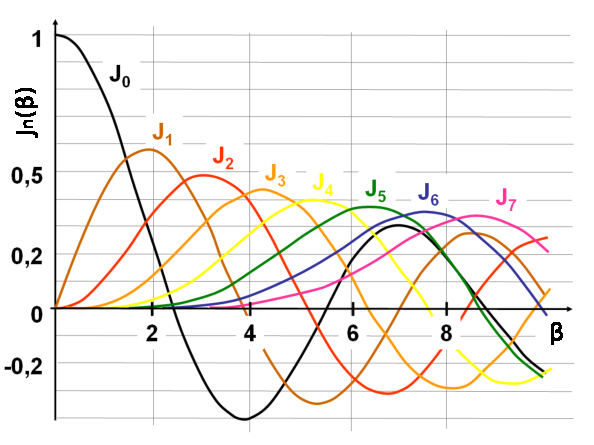
\includegraphics{content/06_amplitudenmodulation/besselfunktionen.pdf}
\end{minipage}
\begin{minipage}{.3\linewidth}
	\textbf{Eigenschaften:}\\
	
	\efbox[linecolor=red]{$J_{-n}(\beta) = (-1)^n\cdot J_n(\beta)$} \\
	
	\efbox[linecolor=red]{$J_{n-1}(\beta) + J_{n+1}(\beta) = \frac{2n}{\beta} \cdot J_n(\beta)$} \\
	
	\efbox[linecolor=red]{$ \sum_{n=-\infty}^{\infty} J^2_n (\beta) = 1$} \\
	
	\efbox[linecolor=red]{$ \beta_n = \Delta T \cdot 2\pi \cdot n \cdot f_c $} \\
	
	$\Delta T$: Zeitverzögerung bezogen auf Grundschwingung ($f_c$) \\
	$n$: n-te Harmonische \\
	
	Tabelle Skript S. 66 bzw. 258 ff.
\end{minipage}

\subsubsection{Bandbreite Einton-Winkelmodulation S. 67}
Theoretisch unendliche Bandbreite \\
Praktisch approximation nach Carson: \efbox[linecolor=red]{$B_{ST} = 2 \cdot (\Delta f+f_m) = 2 \cdot (\beta + 1) \cdot \frac{\omega_m}{2\pi}$} (min. \qty{98}{\%} der Signalleistung)\\
\includegraphics{content/06_amplitudenmodulation/bandbreite.pdf}

\subsubsection[Bandbreite für beliebige m(t)]{Bandbreite für beliebige $m(t)$ S. 67}
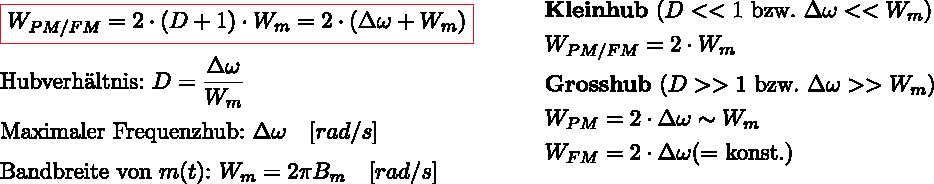
\includegraphics{content/06_amplitudenmodulation/bandbreiteBeliebigem.pdf}

\subsubsection{Realisierung}
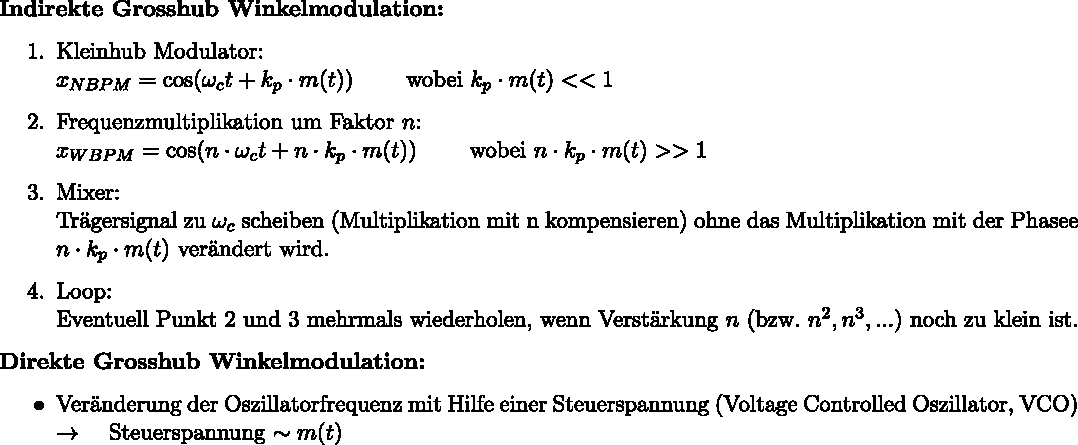
\includegraphics{content/06_amplitudenmodulation/realisierungGrosshubWinkelmod.pdf}

\subsubsection{Demodulation}
\paragraph{Phase Locked Loop (PLL)}
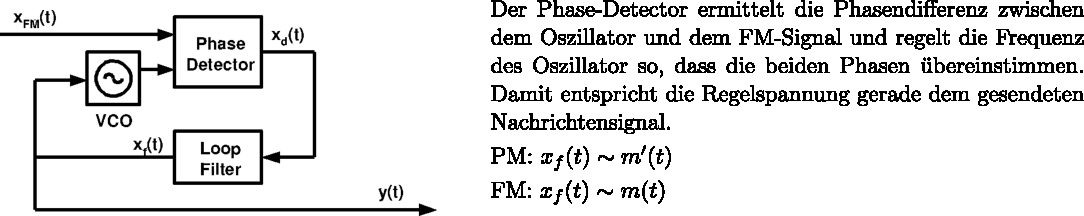
\includegraphics{content/06_amplitudenmodulation/PLLdemod.pdf}

\paragraph{Frequenz-Diskriminator}
Die Amplitude des Ausgangssignals eines Frequenz-Diskriminators ist proportional zur Momentanfrequenz des Eingangssignals. $\rightarrow y_d(t) = k_d \cdot \varphi'(t)$ \\
\textbf{PM:} $y_d(t)=k_d\cdot k_p \cdot m'(t)$ \\
\textbf{FM:} $y_d(t) = k_d \cdot k_f \cdot m(t)$

\subsubsection{FM Empfänger S. 68}
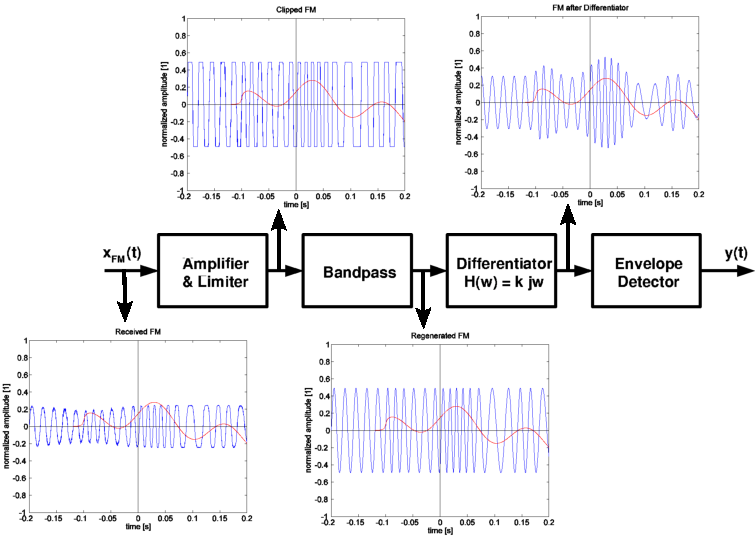
\includegraphics{content/06_amplitudenmodulation/FMreceiver.pdf}